DIVIDE TO image acquisition, reconstruction, postprocessing/rendering
ALSO FURTHER AS theory, previous work, previous usage

Close range photogrammetry, stereopsis, isolated object, camera resectioning


previous usage in:

	rockstar games / la noire; camera pairs

	polar express / sony imageworks

	ea sports / faro


surface vs motion capture

lab environment

other uses - street view, autom driving, geodetic systems

% Aikaisempi tutkimus
\section{Background}

(Should the subsections here be separated into several other sections instead of a single big ``background''?)

(corresponding problems in e.g. autonomous driving or harvester machines?)

(any point in outdoor methods?)

Pairs vs overlap? bradley: pairs

NASA cams

Perf of cloth animation capture

(Crosseyed stereoscopy, how works)

Weak perspective x=fX/Z
Ideal pinhole model projects an image upside down on its film.

\subsection{Imaging} \label{sec:imaging} % {{{
%In addition to multiple cameras at different locations and poses, an uniform lightning is also required to minimize specular difficulties in the texture.

Digital stereo vision in the end analyses digital images; this section introduces the basic image acquisition steps and concerns that affect reconstruction quality. Cameras are never ideal, and practical algorithms take lens imperfections into account (e.g. \cite{opencv}). Images are commonly taken with digital cameras that project a three-dimensional view from a single viewpoint to an image plane, and finally to a discrete grid of numerical values that describe light intensities.

Practical details, such as depth of field, sharpness, aberrations and others are not considered, as they vary greatly depending on the used hardware and are out of scope of this work.
It suffices to say that in a practical system the choice of good optics is a key to good quality reconstruction.
Accuracy and errors depend on not only decidable physical parameters of a stereo imaging rig, such as camera positioning, but also on e.g.~physical construction errors, lens imperfections, camera sensor noise, image compression and algorithmic accuracy. \cite{hollsten2013imagequality, kyto2011method,rieke2009evaluation}.

%In addition to plain photographic cameras, reconstruction can be done using e.g. laser scanners or light field cameras. Those are not covered in this work.

\subsubsection{Pinhole camera}

\simplegfx{h}{0.6\textwidth}{pinhole-camera}
{Pinhole camera principle. The box represents a camera; image seen through the small hole is formed to the plane on its back, rotated upside down.}

A physical camera is in its simplest form modeled as a pinhole camera; an ideal device that projects an image upside down on its film through a small aperture.
Illustration given in image \ref{fig:pinhole-camera}.
In computer vision, this projection is given as a $3 \times 4$ matrix, when homogeneous coordinates are used.
Homogeneous coordinates add an extra dimension to the interpretation of coordinates and each point becomes a line that crosses the origin in a dimension one higher than the original.
In addition, several vector operations become more convenient to manipulate. \cite{hartley03multiview,heyden2005multiple}

The pinhole model (or, perspective projection) states that the world point $(x, y, z)$ is projected to the image plane ($f$ units away from the origin) at $(u, v)$:

\begin{equation}
\begin{pmatrix}
u \\ v
\end{pmatrix}
=
-\frac{f}{z} \begin{pmatrix}
x \\ y \\ z
\end{pmatrix}
\end{equation}

Light rays travel through the pinhole camera's aperture to the image plane that is $f$ units behind the pinhole.
The result can be derived from similar triangles with a common vertex at the aperture.
Sometimes the sign is inverted, which results in a plane between the pinhole (i.e.~camera origin) and the actual point, where the image is not rotated; this can be more convenient to analyse.
\cite{hartley03multiview}

Setting the camera to origin and using homogeneous coordinates, the mapping is given with a camera matrix as

\begin{equation}
\begin{pmatrix}
u \\ v \\ 1
\end{pmatrix}
=
\begin{pmatrix}
x \\ y \\ z/f
\end{pmatrix}
=
\begin{pmatrix} \label{eq:cmat}
	1 & 0 & 0 & 0 \\
	0 & 1 & 0 & 0 \\
	0 & 0 & 1/f & 0
\end{pmatrix}
\begin{pmatrix}
x \\ y \\ z \\ 1
\end{pmatrix}
\end{equation}

The camera position and rotation in a global coordinate frame can be encoded in a matrix so that the point $(x,y,z)$ in global coordinate frame is first transformed relative to the camera's origin; section \ref{sec:coord} discusses this in more detail.

% }}} imaging

\subsubsection{Optics} % {{{

In practice, no actual camera works ideally; imperfections in the lenses project points to positions that differ from those predicted by straight lines in this linear case.
Lens distortions deviate the rays, and no system is in perfect focus, so that one light ray spreads out as a circle.
In reconstructing, methods that estimate the points and minimize errors are used, as no model predicts the camera perfectly.

Construction of optical systems is well studied. \cite{kingslake1989history}
Actual camera lenses consist of not only a single glass element but many, especially in the case of zoom lenses. In this work, the inner workings of these systems are ignored and equations assume a simple projective model, which is a safe assumption when the image is in focus.

The following equation applies for a thin lens while capturing sharp images:

\begin{equation}
	\frac{1}{a} + \frac{1}{b} = \frac{1}{f} \label{eq:focal}
\end{equation}

where f is the focal length of the lens, a is the distance between the lens and the film, and b is the distance between the lens and the imaged source. Figure \ref{fig:focal} example.

% TODO: fig:focal

%The focal length has a direct influence to field of view, as given in figure TODO. Longer focal length (long-focus lens, often referred to as telephoto lens) results to a more zoomed in picture, as opposed to a wide-angle lens. 

All practical optical systems (lenses) introduce some non-linear distortion that affects the performance of the ideal pinhole model.
Common distortions are the purely radial so-called barrel and pincushion distortions, where the magnification is a nonlinear function of image ray distance from the center of the lens. % XXX brown model somewhere here
Fisheye lenses are commonly known to have this kind of effect.
Tangential distortion is less common, particularly in great magnitudes, and is often ignored. Its cause is small misalignments in separate elements in a single optical system; lenses being offset from each other and not parallel to the image plane. \cite{kingslake1989history}

Wilson \cite{wilson2004anton} discusses optical systems' relation to depth of field, focus and distortions.

It should be noted that the nonlinear optical distortions are different from the inevitable perspective projection distortion that happens when projecting a 3D scene to a 2D plane, which is taken into account in the reconstruction.
Perspective distortion refers to the illusion that actual parallel lines would not be parallel in a projected image. \cite{SOMEONE}

\simplefig{h}{%
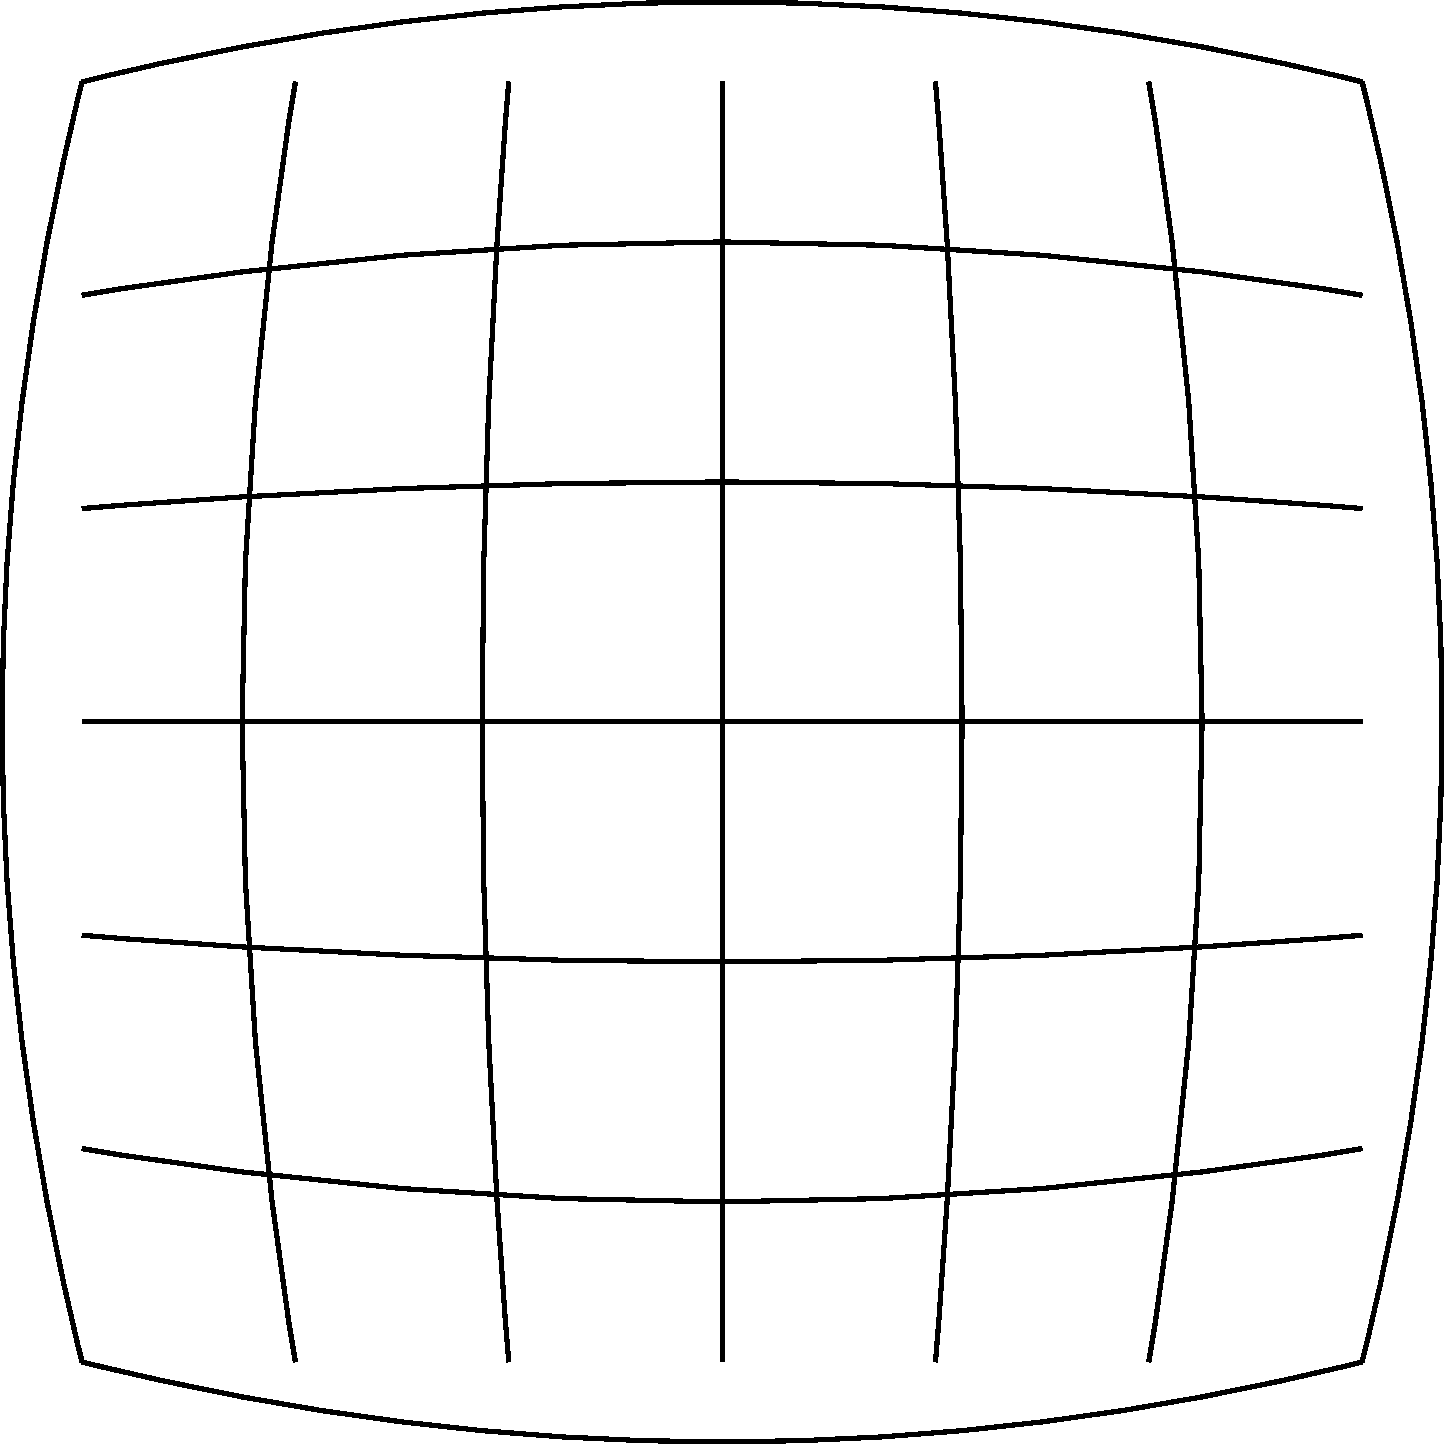
\includegraphics[width=0.2\textwidth]{gfx/barrel-distortion}
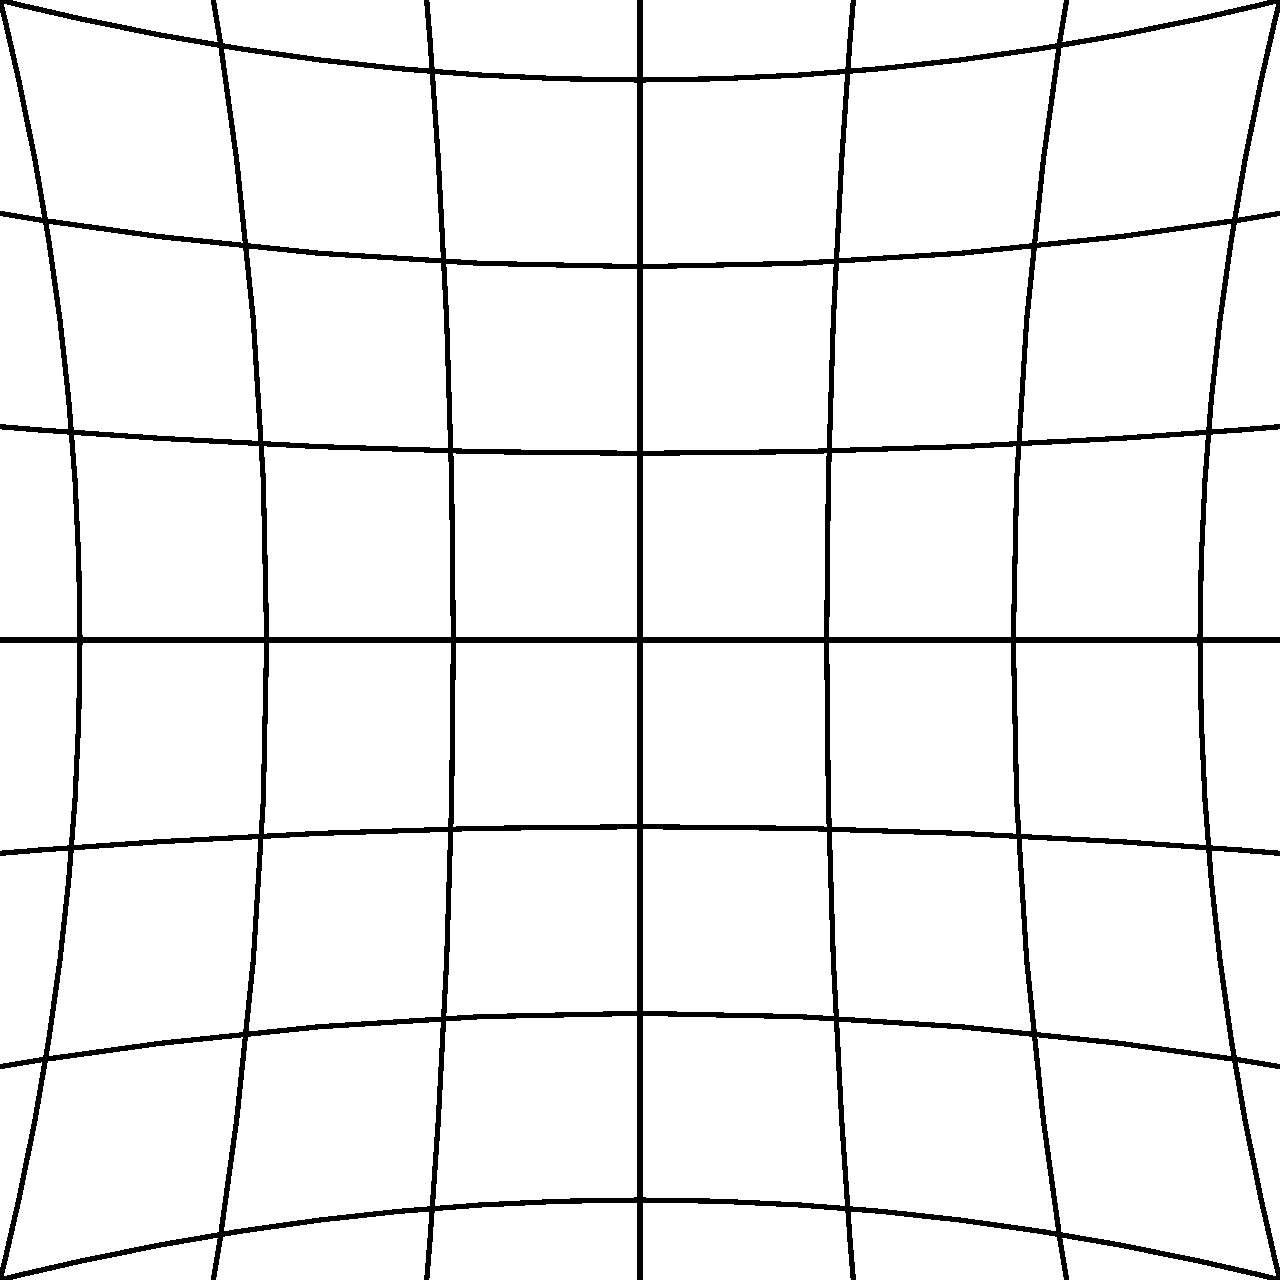
\includegraphics[width=0.2\textwidth]{gfx/pincushion-distortion}
}{fig:distortions}
{Barrel (left) and pincushion distortions that would show up in an image of a grid of straight lines. For a lens with no distortion, the lines would not be curved.}

Distortion should be corrected in software, as the following stereo algorithms assume that the images are free of nonlinear errors, i.e. straight lines in the world should remain straight in 2D images after the projective transformation.
%In particular, image rectification (discussed later in \ref{sec:rectification} won't work if this straightness does not remain; the assumption that similar features should be found on horizontal lines wouldn't hold on distorted images. \cite{hartley03multiview} 

The radial correction used by the OpenCV library to create a new image of the original pixel values at new positions \cite{opencv} is % FIXME brown model

\begin{align}
	x_{corr} &= x(1 + k_1 r^2 + k_2 r^4 + k_3 r^6)\\
	y_{corr} &= y(1 + k_1 r^2 + k_2 r^4 + k_3 r^6)
\end{align}

% (XXX some software does this in a different way (inverse of this, maybe?)

% TODO: illustrate pixel movements, such as in a vector field likein matlab toolbox

Trucco and Verri \cite{trucco1998introductory} use only the two first coefficients. For tangential distortion:

\begin{align}
x_{corr} &= x + (2 p_1 x y + p_2 (r^2 + 2 x^2))\\
y_{corr} &= y + (2 p_2 x y + p_1 (r^2 + 2 y^2))
\end{align}

$x$ and $y$ are the original coordinates in the distorted image, $x_{corr}$ and $y_{corr}$ are the corrected ones, $k_1$, $k_2$, $k_3$, $p_1$ and $p_2$ are coefficients specific to the distortion, and $r$ equals to the distance to image center located at $(x_c,~y_c)$:

\begin{equation}
r = \sqrt{(x - x_c)^2 + (y - y_c)^2}
\end{equation}

%---

Perspective distortion something something viewer location. Normal TV is usually watched at the distance of twice the screen diagonal. At this location, the scene looks normal when taken with a normal lens. A wide-angle scene then looks normal when viewed at a nearer distance. \cite{wilson2004anton}

% 14:01:55 <naavis> Kai sillä yritetään emuloida sitä, että katsojan paikalta se leffan kuvakenttä vastais sitä että valkokankaan tilalla on ikkuna.

% TODO: custom tikz for exactly specified parameters in barrel/radial

TODO: example pic of a fisheyed image and undistorted one.

% \subsubsection{Aperture}

A few words about aperture size, pixel size, diffraction limits, airy disks, circle of confusion, rayleigh limit

a real lens system with several individual elements

stabilisation lens

% }}}

\subsubsection{Image sensors} % {{{

compare to film

photons in, electrons out

array

Microlenses/microfacets

CCD (Charge-coupled Device)

Global shutter

CMOS (Complementary Metal-Oxide Semiconductor)

Cheaper, rolling shutter: reading the pixels out happens linearly

General image quality (noise etc.)

image stabilisation

dust reduction with vibration

%\subsubsection{Bayer filter}

\simplefig{h!}{\bayer{0.7}}{fig:bayerpattern}
{A small subsection of the repeating Bayer pattern, not drawn fully for better visualization. Each square is a single pixel; the grey area represents the image sensor. The gap between pixels is nonzero.}

Physical pixels cover less than the full area of a sensor, as there are gaps between them.

% }}}

\subsubsection{Shutter} % {{{

Mechanical vs. electrical. varying ccd charge time. mechanical moves parts and is slow, wears out. ccd shutter.

Shutter vs frame rate. More discussed in the section \ref{sec:video}. Shutter duration that exposes half of the frame time is common in professional motion pictures \cite{wilson2004anton}. While the shutter is closed, the film advances to next frame (in mechanical cameras). Blur makes the human mind think that the movement is smooth. When sampling for 3D reconstruction, the ideal shutter speed would be infinitesimally fast to reduce blur. Movement in between is then interpolated.

Flash visibility, short flash, flash shared to two frames, X-sync, ISO speed

Image upside down on the sensor, curtain goes physically from top to bottom

moving the curtain back up, springs? too much detail.

Shutter lag (auto exposure/focus even in manual mode maybe?); consistent or not? sensor sensitivity initing lag?

% }}}

\subsubsection{Light sources} % {{{

Area lights, flood flashes around the target

As much light as possible but eyes gonna hurt

dark contact lenses if available (remedy)

bodies' own flashes maybe not uniform enough; too many flashes i guess

softbox or umbrella

light power vs. area, specular lobe and surface properties

%\subsubsection{Specular highlights}

Polarization filter

% }}}

\subsubsection{Image download} % {{{

USB hub(s) because N cameras, single laptop

speed calculations, 20+ MB RAW vs fps vs camera buffers vs usb bandwidth vs separate hubs

usb bulk transfer protocol overhead! how many percents?

% }}}

\subsection{Video}

Video is consecutive, ordered pictures displayed one after another.

Hox ALL-I (intra) vs. IPB (intra-predict-bidirpredict)

\subsubsection{Frame rate effects}

More fps = better movement stopping (less motion blur), need also more light or more sensitive sensors. More sensitivity often means also more noise. Noise vs. motion blur trade-off.

Interlaced video = twice the amount of *pictures*, two pictures per frame

Film: 24 FPS traditionally

PAL. 25 FPS (50 Hz line current frequency in Europe)

NTSC. 30 FPS (60 Hz line current frequency in the US)

Actual FPS in camcorders is slowed down by a factor of 1.001 because of historical reasons relating to black and white / color TV backwards compabilities [REF].
30 and 24 FPS refer often actually to approximately 29.970 and 23.976 FPS, respectively.

24 frames per second is often transformed to 30 by carefully repeating some frames [REF].

Externally triggered cameras can be configured to record at any arbitrary speed, as long as it's in the limits of the camera speed capabilities.

\subsubsection{Frame rate vs. shutter speed}

Picture:

\begin{verbatim}

   those bars are actually just 1 pixel markers when shutter opens
   v   v   v ...

shutter
speed
1/30   |---|---|---|---|---|---|---|---|---|--- full block
1/60   |-- |-- |-- |-- |-- |-- |-- |-- |-- |--
1/90   |-  |-  |-  |-  |-  |-  |-  |-  |-  |-

   0   1   2   3   4   5   6   7   8   9

30 FPS, 10 frames = 1/3 s
\end{verbatim}

Nyquist-Shannon sampling theorem, what happens when shutter is closed, motion stopping, how eyes like blurred fast motion (more information about movement, less precise by time) [CITE slowmovideo]

\subsubsection{Multi-camera synchronization}

Multi view imaging poses lots of challenges, sync is an important one

Time offset / drift / jitter / lockstep

Offset: Different cameras do not start recording immediately at the same time, which results in one or more cameras being a little late at every frame.

Drift: A camera does not record at exactly the advertised speed, e.g. one camera's internal clock is sligtly faster than that of another.

Jitter: the difference between frames for a same camera might not be exactly the same during recording, but a more or less random delta time is added to each delay.

Le pic:

\begin{verbatim}
Offset

cam A  |   |   |   |   |
cam B   |   |   |   |   |
   0t  1t  2t  3t  4t time -->


Drift

normal   |   |   |   |   |   |   |
drifting |    |    |    |    |    |
	 0t  1t  2t  3t  4t  5t  6t time -->


Jitter

normal   |   |   |   |   |   |   |
jitterin |    |  |   | |      |    |
	 0t  1t  2t  3t  4t  5t  6t time -->
\end{verbatim}

In the scope of this paper, we consider drift and jitter negligible.
Offset may be recovered by several means.
Often used techniques are starting flash (does not need an audio track) [REF], clapperboard [REF], strobe sync'd to fps, genlock.

TODO: investigate if the errors have been researched or if they are meaningful at all.


\subsection{Camera selection}

Good: Smaller sensor; smaller focal length; closer to target; less camera position disparity; smaller rig

Image quality: lens quality, sensor size, pixel count, lightning

Common sensor sizes in dslr cameras

Common sensor sizes in pocket cameras

Canon / Nikon dslr

% http://www.agisoft.ru/forum/index.php?topic=1411.60

lens sharpness, contrast, freq; MTF modulation transfer function for the lens sharpness / perceptual mpix

fixed lens (prime) instead of zoom: more or less lab controlled environment -> target position can be adjusted, zoom would be just more parameters to optimize. focal length is important to know; also, mirror vibration might move the zoom over time.

no anti-shake/image stabilizer  (photogrammetry.doc) in sensor or lens

Rieke-Zapp et al \cite{rieke2009evaluation} address several problems in camera calibration and imaging quality, e.g. mechanical problems blah blah

sensor vibration to remove dust -> sensor position not very fixed (rieke2009)

ring flash bending the lens assembly if attached to it (rieke2009)

\subsubsection{DSLRs}

Intended for single pictures

Mechanical shutter

Big sensor

Shallower DOF

Focal length configurable

Lots of resolution

Memory card speed

gphoto2

No autofocus in general

Easy sync for single image

\subsubsection{Pocket cameras}

Affordable

Small sensor

Decent resolution

Configurability unknown

Manual mode required

Always a zoom lens, bad for calibration


\subsubsection{Camcorders}

Electrical shutter

Ok fps

More features for video

Autofocus (not needed here)

Better (deeper) DOF for video

Usually zoom lens

Consumer devices: affordable

Pro devices: bukkits of money (features; external sync)

Internal hard disk

Interlace vs. progressive recording

\subsubsection{Machine vision cameras}

Well controllable, flexible (in SW terms), still vendor-specific APIs for tuning the settings

External sync

Raw data

Data bandwidth, auxiliary hardware

Expensive

- vendor-specific apis
- probably easier to control
- expensive
- raw images (high bandwidth)
- usually fixed lens
\subsubsection{Depth cameras}

In addition to stereo depth...

Active measurement (difficult to use several)

Laser rangers

IR patterns and an IR camera (Kinect)

\subsubsection{(Light field cameras)}

Lytro (NOPE)

\subsubsection{Hybrid systems}

Use several camera types at the same time? depth camera for more reliable and fast measurements?


\subsection{Hardware}

\subsubsection{Image storage}

\subsubsection{Transport buses and cabling}

\subsubsection{(Mechanical something)}

Integral memory cards / disks, offline usage

USB2

USB3

Firewire

GigE

Camera Link

libgphoto2

\subsection{Image acquisition steps}

Guidelines for successful pictures/video

\subsection{Static 3D reconstruction}

TODO: combine and structure better the following flattened section list

\subsubsection{Imaging methods}

Light field, structured light, laser scanner

- every Nth frame fre of patterns for texture extraction (zhang snavely curless 2004)
- maybe not fast enough with common cameras

\subsubsection{Camera calibration}

Calibration is often specified with a camera projection matrix, or several separate matrices. It may be convenient to store intrinsics and extrinsics separately if the intrinsic matrix is constant for several pictures, for example.

Triangulation or reconstruction of the scene structure given by image pair(s) is usually done on the base of a known relationship between the cameras. Such relationship, known as calibrating the cameras, can be automatically determined, given by X corresponding points that can be distinguished in each image and matched [?]. Commonly the points are particular \emph{features}, commonly very noticiable edges or corners, found with an algorithm such as SIFT [?], SURF [?] or Harris corner detector [?].

Automatic calibration tools rely on an amount of feature pairs of which the best matches are found, or a known pattern, such as a planar checkerboard pattern [chuan; zhang] whose features are also distinguished with a similar algorithm but a priori knowledge of the object structure is used for precise calibration. These usually need several pictures taken with the same camera from different poses.

The checkerboard calibration step can also measure optical distortion at the same time; e.g. opencv[?], matlab camera calib toolbox [?]

TODO Figure: show extrinsic in matlab cam calibs, nice pics (both cam and world centered)

Single three-dimensional calibration object is also sufficient blbl

One possible way is direct linear transform (DLT) [hartley/zisserman multiviewgeom]: Solve whole projection matrix instead of individual parameters, decompose projection to intrinsics and extrinsics. For each projected point $\vec x$ from 3d point $\vec X$,

\[
	\vec x = M \vec X
\]

and construct N of these equations and solve for $M$.

Methods that dig the matrix out of a single image have certain restrictions, and won't work if e.g. seven points lie on the same plane [longuet-higgins etc.]

XXX see below. Intrinsic, extrinsic. Distortions. Projection matrices. Camera resectioning.

many single planar chessboard pics vs. a single image of an accurate 3d model.

\subsubsection{Normalization}

The scale of values in the equations above affects the precision [hartley, in defense of .., h+ziss]. A similarity transform can be used to modify the values to a more consistent range.

Translate centroid to the origin, scale so that average becomes sqrt 2.


\subsubsection{Coordinate systems and transforms}

Homogenous point description here, [dubrofsky] homography estimation is nice, also refer hartley/zisserman

Homography definition (mapping of points and lines in $P^2$) / panorama homography

The imaging process essentially captures a projection to a flat two-dimensional plane of the camera's view.
When relating points between different cameras that view the same scene, their relational positions and rotations must be known.
One of the cameras is often chosen as the origin of a global coordinate frame.
Each three-dimensional point in the world is transformed to the small sensor or film inside the camera, which is then digitized to a discrete two-dimensional grid of pixels. The size of this pixel array (i.e. image) is referred to the camera's resolution.
Figure \ref{fig:TODO} illustrates this transformation chain, which is encoded as the following equation, given a homogenous point (4-dimensional vector) $X$ representing a 3D location described in physical (e.g. metric) coordinates:

\begin{align}
	x_i &= P X\\
	  &= M_2 X_s\\ % X_s on the sensor
	  &= M_2 R T X\\
	  &= M_3 M_4 R T X\\ % R, T camera pose, M_4 to camera sensor, M_3 to pixel coords
\end{align}

$p_i$ 2d pixel in discrete image, $X_s$ on the sensor, $T$ is a simple translation matrix from $\vec t$

Note that the projection $P = M_3 M_4 R T$.

The external camera parameters are called the extrinsics: camera coordinate system position and rotation (heading) in the global space.
Camera position (projection center) blah.
The internal parameters, intrinsics, encode how the image is formed on the sensor: they consist of focal length, sensor size and principal point:
\begin{equation}
	M =
	\begin{pmatrix}
		m_x & \gamma & u_0\\
		0   &    m_y & v_0\\
		0   &        0 & 1
	\end{pmatrix}
	*
	\begin{pmatrix}
		f & 0 & 0\\
		0 & f & 0\\
		0 & 0 & 1
	\end{pmatrix}
	=
	\begin{pmatrix}
		\alpha_x & \gamma   & u_0\\
		0        & \alpha_y & v_0\\
		0        & 0        & 1
	\end{pmatrix}
\end{equation}

For simplicity, we denote $\alpha_x = m_x f$, $\alpha_y = m_y f$. $(u_0, v_0)$ is the image center (or principal point). For square pixels, $m_x = m_y$, and for a non-skewed sensor, $\gamma = 0$, which is often the case.

Le image. Horizontal planar triangle, lines between camera origins etc. lecture11.pdf.

\subsubsection{Binocular disparity}

Essential, fundamental matrices. Correspondence problem. Rectification, undistortion. Epipolar geometry.

(fund generalization of ess.)

(fund and ess. in global and pixel coords)

Two cameras: ideal stereo setup, such as human eyes; cameras are parallel, looking straight and shifted only in the x (or y) axis. Calibration assumed to be known.

Similar triangles:

\begin{align}
	\frac{Z}{T} &= \frac{Z-f}{T - x_l + x_r} &= \frac{Z-f}{T - d}
	ZT - Zd &= ZT - fT
	Z = \frac{fT}{d}
\end{align}


Depth inversely proportional to disparity. Algorithms such as those in OpenCV can compute point clouds from disparity images.

Two or more cameras

(Should this and the next ones be under a "methods for multi view stereo" section?)

\subsubsection{Epipolar geometry}

A point seen by camera A at 3d point P could be anywhere on the line between A's origin and P.
This line is seen as a single point.
From another viewpoint in camera B, this line equals to some line on B's image plane.
The real point must be on that line.
The inverse applies for any point on B and a line on A.
The lines on the image planes are called epipolar lines.


Essential matrix defines how the camera poses differ by the something something points seen by both. $p_l$, $p_r$ 3d points; vectors from camera origins (camera coordinates!) to the same point

\[
	p_l^T E p_l = 0
\]

Le image. lecture11.pdf. O->p dot (O->O' cross O'->p') = 0

Cross product expressed in a skew-symmetric matrix form is
\begin{equation}
\vec a \times \vec b =
\begin{pmatrix}
	 0   & -a_z &  a_y\\
	 a_z &  0   & -a_x\\
	-a_y &  a_x & 0
\end{pmatrix}
\begin{pmatrix}
	b_x\\b_y\\b_z
\end{pmatrix}
= \vec c
\end{equation}


Fundamental matrix relates the corresponding points in stereo images.

Epipole can be interpreted as the location of another camera as seen by other camera.



\subsubsection{Point matching}

%\subsubsection{something fucky}

snake surrounding stuff

visual hull

salient geometric features for matching

\subsubsection{Correspondence and rectification}

In order to triangulate a real point from two or more photos, the location of the point in all images must be known.
Given a pixel in one image, what is the corresponding pixel in another image taken from the same scene?

Rectification is a process that simplifies this search problem by restricting the search to a single dimension.
By aligning the cameras such that their images are coplanar, the search only has to be performed on a line that is parallel to the line connecting the camera centers.
Usually, the calibration between the cameras is known at this point, and foobar.
After rectification, the corresponding lines are axis-aligned (horizontal or vertical) in both images.



\subsubsection{Multi-view stereo}

\subsubsection{Structure from motion}

Structure from motion (SfM) refers usually to recovering the structure of a scene from the motion of a single camera.
For each view, the pose of the camera is determined and the scene structure is extended with the new information in the image.
(pollefeys)

\subsubsection{Bundle adjustment}

\subsubsection{Reprojection errors}

The quality of the reconstruction is measured by reprojecting the 3D points back to the cameras and calculating the distance between the projected and original point.
Minimizing all of the points is very expensive but something something bundle adjustment.

Compare to algebraic, geometric etc.

A common way to handle feature errors is Random Sample Consensus (RANSAC). Random subsets of the sample space is iterated, and samples that do not fit well to a model that is constructed of a smaller set are ignored. The iteration that matches most samples is selected.

Detail calculation (error on surface ~= avg reprojection error?) compute millimeters

Mesoscopic level shape reconstruction

\subsection{Surface fitting}

\subsubsection{Geometry}

Meshlab

build mesh from the point clouds that has been built from the pixels

\subsection{Texture reprojection}

use the registered raster projections to find out best textures and build uv coordinates

\subsubsection{Rendering}

(vipe / visualsfm / kiipeily)

Uv mapping. Manual work. 3d noise removal; ignore points that have no close pair in other clouds.

Rendering: "as usual".

Postprocessing: remodel the mesh (face), see what it would look like. Refine parameters to get a similar output as in the photos (normal map etc.), backproject. Use colors and highpass them; assume uniform lightning and locally uniform texture color (bradley). (Simply a rendering technique, that level of detail in 3D structure might not be needed). Still, structured light and/or shading assumptions [shape from single image cues/shading trucco+verri p.225] done too.


(video: 3d topology different in each frame; most algos do just stills. simple to combine them to a pre-recorded mesh)


\subsection{Tracking}

Kalman

Fiducials / AR

perf of cloth anim capture
\subsubsection{Optical flow}

Long history; several mature commercial video editing products. The Matrix.

Uses: Frame time offset compensation by interpolation (morphing), needs features, direction vector estimation


\subsubsection{2D features}

* SIFT/SURF/Harris feature tracking, reproject

* edgels (edge pixels)

\subsubsection{3D}

*


\subsubsection{Feature / surface tracking}

Pore-level matching, good resolution needed

Many cameras, zoom in to just a part of the target

Markers / markerless

Markers traditional

%http://en.wikipedia.org/wiki/Facial_motion_capture the polar express, beowulf

This work considers markerless capture important, because time-varying texture is important in facial capture (wrinkles from different facial expressions)

Special marker makeup / pre-recording of pore-level texture? Then "good enough" zillion markers and map and deform the mesh?

Corner detector (harris, sift, surf). Color usually not important. Brightness constancy. Repeated texture or no texture (uniform color = bad).

Matching to a priori model

\subsubsection{Kalman}

\subsection{Motion capture}

\subsubsection{4D video}

topologically different 3d models

\subsubsection{Registration}

Combining 3D meshes from multiple viewpoints (cameras/camera pairs). Also e.g. ransac for removing noise. Iterative closest point fitting.


\subsubsection{Morphing}


\subsection{Facial surface capture}

Surface capture of human skin is different from static objects: it stretches and shears in a highly non-predicatable way such that both its local geometry and texture changes.
Traditional methods for tracking rigid objects are thus not viable for high quality.
Some cites here [?] [?]. The deformations can be taken into account with e.g. furukawa etc.

Several 

\subsubsection{Uncanny valley}

\subsubsection{Expression space}

Some techiques [autodesk faceshift, what other] use pre-recorded facial expressions to identify the subject's pose. They suffer from not being able to accurately describe the temporal changes in finest details, but benefit from densely packed parameterization of facial expressions.
A separate mesh is stored as a three-dimensional template for each expression (such as happy or angry) and each frame is encoded, as a linear combination of these individual expressions.
Such feature vectors describe well each possible face, and importantly, they eliminate the need for encoding the movement of each vertex, which can be unnecessarily heavy to compute or store.
The results from this method can easily be mapped to other models than the face of the subject, as it is independent on the actual facial geometry and only uses weights for pre-modeled faces, making it interesting in computer animation.

Compare to Facial Action Coding System (FACS) (Hjortsjö 1969), which parameterizes the face in a group of muscular actions. This is similar to grouping vertices in keyframe animation [?].

Expression tracking / 2d capture

\subsubsection{Rendered facial animation}


\subsection{Preprocessing}

- sync shit

- histogram equalization

- brightness equalization between images


\subsection{Postprocessing}

\subsubsection{Manual work}

so much

\subsubsection{Motion evaluation}
